\documentclass[a4paper]{article} %doctype define
\usepackage[a4paper,hmargin={3cm,2.5cm},vmargin={2.5cm,2.5cm}]{geometry} %setup margins
\usepackage[utf8]{inputenc} %for special character support
\usepackage{graphicx}   %for defining images root folder below
\graphicspath{ {images/} }
\usepackage{hyperref} %link table of content with actual text part

%===============For Code visibility======================
\usepackage{listings}

\usepackage{xcolor} %define custom colors
\definecolor{mygreen}{rgb}{0,0.6,0}
\definecolor{mygray}{rgb}{0.5,0.5,0.5}
\definecolor{mymauve}{rgb}{0.58,0,0.82}
\definecolor{compilerRed}{HTML}{cc0000}

\lstset{
    backgroundcolor=\color{white},      % choose the background color; you must add \usepackage{color} or \usepackage{xcolor}; should come as last argument
    language=[x86masm]Assembler,                    % the language of the code
    basicstyle=\footnotesize\ttfamily,  % the size of the fonts that are used for the code
    % breakatwhitespace=false,            % sets if automatic breaks should only happen at whitespace
    % breaklines=true,                    % sets automatic line breaking
    captionpos=b,                       % sets the caption-position to bottom
    commentstyle=\color{mygreen},       % comment style
    % deletekeywords={...},               % if you want to delete keywords from the given language
    % escapeinside={\%*}{*)},             % if you want to add LaTeX within your code
    % extendedchars=true,                 % lets you use non-ASCII characters; for 8-bits encodings only, does not work with UTF-8
    firstnumber=1,                      % start line enumeration with line 1
    numbers=left,                       % where to put the line-numbers; possible values are (none, left, right)
    numberstyle=\tiny\color{mygray},    % the style that is used for the line-numbers
    numbersep=7pt,                      % how far the line-numbers are from the code
	frame=single,                       % code snippet frame, t-> top, b->bottom, l->left, r->right, single-> all around
	tabsize=4,                          % tab = (tabsize) * space
    columns=flexible,                   % two options, fixed or flexible
    keepspaces=true,                    % keeps spaces in text, useful for keeping indentation of code (possibly needs columns=flexible)
    morekeywords={*,MVI, DAD, INX, DCR, LXI},               % if you want to add more keywords to the set
    rulecolor=\color{black},            % if not set, the frame-color may be changed on line-breaks within not-black text (e.g. comments (green here))
	showspaces=false,                   % show spaces everywhere adding particular underscores; it overrides 'showstringspaces'
    showstringspaces=false,             % underline spaces within strings only
    showtabs=false,                     % show tabs within strings adding particular underscores
    stepnumber=1,                       % the step between two line-numbers. If it's 1, each line will be numbered
    stringstyle=\color{mymauve},        % string literal style
    title=\small\lstname,               % show the filename of files included with \lstinputlisting; also try caption instead of title
	% keepspaces,
	keywordstyle=\color{blue},           % keyword style    
    morecomment=[l][\color{compilerRed}]{\#}
}

\begin{document}


\begin{titlepage}
    \begin{center}
        \vspace*{1cm}
 
        \huge
            \textbf{Microprocessor Lab Report}\\
        \vspace{1cm}
        \large
            \textbf{Abhiroop Mukherjee}\\
            \textbf{Enrl. No: 510519109}\\
        \vspace{1cm}
        
\includegraphics[width=0.4\textwidth]{IIESTS-Logo.png}\\
        \vspace{1cm}
        \normalsize
        Department of Computer Science and Technology\\
        Indian Institute of Engineering Science and Technology, Shibpur 
 
        \vfill               
    \end{center}
 \end{titlepage} %Title Page

\pagenumbering{roman}
\setcounter{tocdepth}{1} % only allow 1 nests
\tableofcontents
\newpage
\pagenumbering{arabic}
\setcounter{page}{1}
% ==================MAIN TEXT========================
\section[Find out the sum of the first 30 natural numbers]{Assignment 1} %[toc content]{text content}
    \subsection{Objective}
        Find out the sum of the first 30 natural numbers.
    \subsection{Tool/Experimental setup considered}
        \begin{itemize}
            \item Jubin's 8085 Simulator
        \end{itemize}
    \subsection{Procedure}
        We know that
        \[1 + 2 + 3 + ... + 29 + 30 = \frac{30 \times 29}{2} = 435 =  01D1H\]
        This result is not possible to store in a single register, so we need to use register pair to store the result.
    \subsection{Program}
        \lstinputlisting[caption=assembly program to find sum of the first 30 natural numbers]{./../Programs/Assignment 1/1_1_sum till 30.asm}
    \subsection{Experimentation}
        \begin{center}
            \fbox{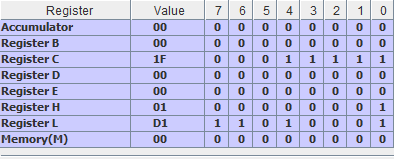
\includegraphics[width=0.7\textwidth]{Assignment 1/1_sum_till_30/registor.png}}\\
        \end{center}
    \subsection{Conclusion}
        We see that after the execution of program, the data stored in HL register pair is 01D1H, which is the hexadecimal value of 435.\\
        Hence the Program is working as expected
\newpage

\section[Find minimum and maximum number in 10-byte unsigned array]{Assignment 2} %[toc content]{text content}
    \subsection{Objective}
        From an array of 10-byte size integers (unsigned) find out the maximum and minimum.
    \subsection{Tool/Experimental setup considered}
        \begin{itemize}
            \item Jubin's 8085 Simulator
        \end{itemize}
    \subsection{Procedure}
        The idea is to linearly iterate through all the values of the arr, and update the register for minimum(C) and maximum(B) values.
    \subsection{Program}
        \lstinputlisting[caption=assembly program to find minimum and maximum number in 10-byte unsigned array]{./../Programs/Assignment 1/1_2_min-max of 10 size array.asm}
    \subsection{Experimentation}
        \begin{center}
            \fbox{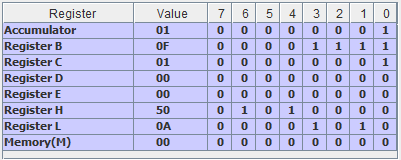
\includegraphics[width=0.7\textwidth]{Assignment 1/2_min-max-10-elem/register-config.png}}\\
        \end{center}
    \subsection{Conclusion}
        We see that that after program execution, B has the maximum value of array(F), and C has the minimum value of the array(C).\\
        Hence the Program is working as expected
\newpage

\section[Delay Procedure]{Assignment 3} %[toc content]{text content}
    \subsection{Objective}
    Write a routine that produces a delay. The delay value must be passed to register pair DE.
    \subsection{Tool/Experimental setup considered}
        \begin{itemize}
            \item Jubin's 8085 Simulator
        \end{itemize}
    \subsection{Procedure}
        Idea is to define DE as a very big value (say FFFF), and decrement it in a loop till DE becomes 0 to produce delay in execution.
    \subsection{Program}
        \lstinputlisting[caption=assembly program to produce delay]{./../Programs/Assignment 1/1_3_delay.asm}
    % \subsection{Experimentation}
    %     \begin{center}
    %         \fbox{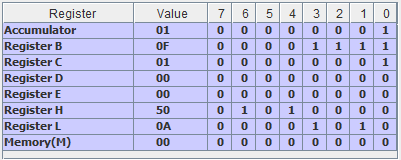
\includegraphics[width=0.7\textwidth]{Assignment 1/2_min-max-10-elem/register-config.png}}\\
    %     \end{center}
    \subsection{Conclusion}
        We see that the code runs for sometime, then it completes it's execution, signifying that the delay function worked and delayed execution of CPU for some time.\\
        Hence the Program is working as expected
\newpage

\end{document}